\chapter{Método de Trabajo}
\label{chap:metodo}
\label{chap:metodologia}

%haz un check de los acrónimos

\section{\acf{PUD}}

\drop{E}{n} \cite{rumbaugh_jacobson_pud} se define el \acf{PUD} como un proceso de desarrollo
de software. A su vez, un proceso de desarrollo de software es el conjunto de
actividades necesarias para transformar los requisitos de usuario en un sistema
software (véase figura \ref{fig:proc-software}). 

\begin{figure}[!h]
  \begin{center}
    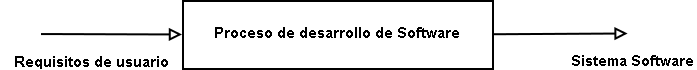
\includegraphics[width=1.0\textwidth]{/proceso-software.png} 
    \caption{Proceso Software \cite{rumbaugh_jacobson_pud}}
    \label{fig:proc-software}
  \end{center}
\end{figure}


El \acs{PUD} está basado en \textit{componentes}, lo que significa que el
software en construcción está formado por componentes interconectados a través de
interfaces bien definidas. 

Para diseñar y desarrollar todos los artefactos de un sistema software, el \acs{PUD}
utiliza un lenguaje unificado de desarrollo denominado \acf{UML}. Se puede consultar más información sobre \acs{UML} en \cite{rumbaugh_unified_2004}. 

\cite{rumbaugh_jacobson_pud} define las principales características del
\acs{PUD} en: 

\begin{enumerate}
\item Dirigido por casos de uso.
\item Centrado en la arquitectura.
\item Iterativo e incremental.
\end{enumerate}

\subsection{Características del Proceso Unificado de Desarrollo}

\subsubsection{Dirigido por casos de uso}

La finalidad de un sistema software es proporcionar servicio a los usuarios
\cite{rumbaugh_jacobson_pud}. Estos usuarios pueden ser tanto humanos como otros
sistemas, luego el término \textit{usuario} se refiere a toda aquella entidad
que interactúa con el sistema que se está desarrollando. Es una interacción
concreta la que da nombre al concepto \acf{CdU}.

En \cite{rumbaugh_jacobson_pud} se define \textbf{caso de uso} como un fragmento
de funcionalidad del sistema que proporciona al usuario un resultado
importante. 

La función de los casos de uso es representar los requisitos funcionales del
sistema. Al conjunto de todos los casos de uso se le denomina \textbf{modelo de
  casos de uso}. \cite{rumbaugh_jacobson_pud} define al modelo de casos de uso
a aquel formado por casos de uso, actores y sus relaciones. Un modelo de casos de
uso define la funcionalidad de todo el sistema, así pues representa todos los
escenarios de interacción posible entre el usuario y el sistema. 

\cite{rumbaugh_jacobson_pud} advierte que si bien es cierto que los casos de uso
guían el proceso no deben ser desarrollados de manera aislada, pues hay que
considerar la arquitectura del sistema. \textit{Los casos de uso guían la
  arquitectura del sistema y la arquitectura del sistema influye en la selección
  de los casos de uso}. 

Esto sugiere que existe un proceso de \textbf{maduración} tanto de arquitectura
como del modelo de casos de uso a medida que avanza el ciclo de desarrollo. 
 

\subsubsection{Centrado en la arquitectura}

Al igual que en la construcción de edificios, el papel de la arquitectura de
software se puede contemplar desde diversos puntos de vista, tales como
estructura o servicios \cite{rumbaugh_jacobson_pud}. En una arquitectura
software la visión incluye aspectos estáticos y dinámicos. Así pues una
arquitectura surge de las necesidades y refleja los casos de uso, pero también
se ve influida por otros muchos factores (plataforma, marcos de trabajo,
interfaces gráficas, requisitos de rendimiento o fiabilidad, etc.). 

\cite{rumbaugh_jacobson_pud} denota que la relación existente entre casos de uso
y arquitectura debe ser la siguiente: 

\begin{enumerate}
\item Los casos de uso deben encajar en la arquitectura cuando se llevan a cabo.

\item La arquitectura debe permitir el desarrollo de todos los casos de uso
  requeridos y permitir una evolución en paralelo. 
\end{enumerate}

De esta manera los casos de uso representan la función del sistema mientras que
la arquitectura define la forma de dicho sistema.

Según \cite{rumbaugh_jacobson_pud} el arquitecto:

\begin{enumerate}

\item Realizará una versión inicial de la arquitectura, comenzando por la sección del
  sistema que no es específica de los casos de uso pero debe mantener en
  perspectiva de éstos antes de comenzar la creación del esquema arquitectónico.

\item Trabajará con un subconjunto de los casos de uso que represente las
  funciones clave del sistema. Estos casos de uso deben especificarse en detalle y
  se realizará en términos de subsistemas, clases y componentes. 

\item A medida que los casos de uso se especifican y desarrollan se
  descubren nuevos aspectos de la arquitectura, lo que implica una maduración de
  los casos de uso. 

\end{enumerate}


\subsubsection{Iterativo e incremental}

Cuando se aborda el desarrollo de un producto software se asume que supondrá un
gran esfuerzo en términos económicos y temporales. Así pues resulta práctico
dividir el trabajo en partes más pequeñas que se denominan iteraciones. Cada
iteración obtendrá como resultado un incremento y dicho incremento se traducirá
en una pequeña mejora o avance en el desarrollo del producto. En
\cite{rumbaugh_jacobson_pud} se remarca la necesidad de establecer iteraciones
\textit{controladas}, es decir, iteraciones que deben ser previamente
seleccionadas y ejecutadas de forma planificada como si fuesen proyectos más
pequeños. 

Para llevar a cabo este control, el desarrollador basa la selección en dos
factores \cite{rumbaugh_jacobson_pud}: 

\begin{enumerate}
\item La iteración tratará un grupo de casos de uso que en conjunto ampliarán la
  utilidad del producto desarrollado. 
\item La iteración tratará los riesgos más importantes. 
\end{enumerate}

Puesto que cada iteración se considera un mini-proyecto, tomarán como punto de
partida los casos de uso y después desarrollará el trabajo según  los flujos: 

\begin{enumerate}
\item Análisis
\item Diseño
\item Implementación
\item Pruebas
\end{enumerate}

\cite{rumbaugh_jacobson_pud} aclara que al final de cada iteración no se tiene
por qué tener un incremento necesariamente aditivo puesto que en las primeras
fases del ciclo de vida los desarrolladores pueden tener que realizar tareas de
reemplazo de diseño (los más superficiales por los más sofisticados). No
obstante en las fases posteriores los incrementos suelen ser aditivos. 

Según \cite{rumbaugh_jacobson_pud}  el desarrollador durante una iteración del
\acs{PUD} debe realizar las siguientes tareas: 

\begin{enumerate}
\item Identificar y especificar los casos de uso más relevantes. 
\item Crear un diseño siguiendo la arquitectura seleccionada. 
\item Implementar el diseño mediante componentes. 
\item Verificar que los componentes satisfacen los casos de uso. 
\end{enumerate}

Todo ello ciñéndose al orden lógico de las iteraciones para economizar recursos
y lograr el objetivo. Es habitual que surjan problemas inesperados y sea
necesario realizar adaptaciones a los nuevos problemas, pero siguiendo un plan
los beneficios son significativos:


\begin{enumerate}
\item El coste del riesgo se reduce a solo un incremento del proceso. Si una
  iteración debe repetirse, la organización sólo perdería el esfuerzo empleado
  en la iteración en concreto. 
\item Se reduce el riesgo de retrasos en la entrega del producto mediante la
  identificación de riesgos en las fases más tempranas. 
\item Puesto que los desarrolladores trabajan de manera más eficiente se
  consigue incrementar el ritmo del esfuerzo de desarrollo. 
\item El cambio de requisitos por parte de los usuarios no es acentuado, debido
  a que los requisitos se van refinando durante las iteraciones. 
\end{enumerate}


\subsection{Ciclo de vida del Proceso Unificado de Desarrollo}

\subsubsection{Modelo del \acs{PUD}}

El \acs{PUD} se repite a lo largo de una serie de ciclos que constituyen la vida
de un sistema y cada ciclo concluye con una versión del producto
\cite{rumbaugh_jacobson_pud}. 

Cada ciclo está constituido por cuatro fases y cada fase a su vez se divide en
iteraciones como ilustra la figura \ref{fig:ciclos-pud}.  


\begin{figure}[!h]
  \begin{center}
    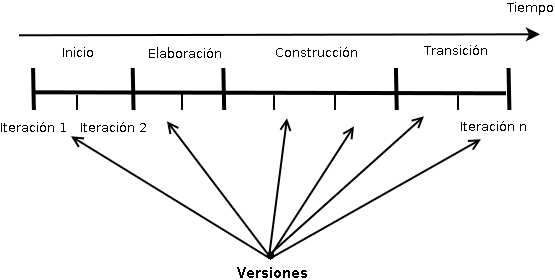
\includegraphics[width=0.8\textwidth]{/ciclos.png} 
    \caption{Ciclo con fases e iteraciones \cite{rumbaugh_jacobson_pud}.}
    \label{fig:ciclos-pud}
  \end{center}
\end{figure}


En cada ciclo se produce una nueva versión del sistema, siendo una versión un
producto preparado para su entrega. El entregable a su vez consta de un cuerpo
de código fuente además de manuales y productos asociados a su
funcionamiento. El producto terminado incluirá los requisitos, casos de uso,
especificaciones no funcionales y casos de prueba, incluyendo el modelo de la
arquitectura y el visual. 


Para llevar a cabo los ciclos del \acs{PUD} los desarrolladores necesitan todas las
representaciones del producto software. Estas representaciones del producto se
denominan \textbf{Modelo del Proceso Unificado} (véase figura \ref{fig:ciclo-fin}).

\begin{figure}[!h]
  \begin{center}
    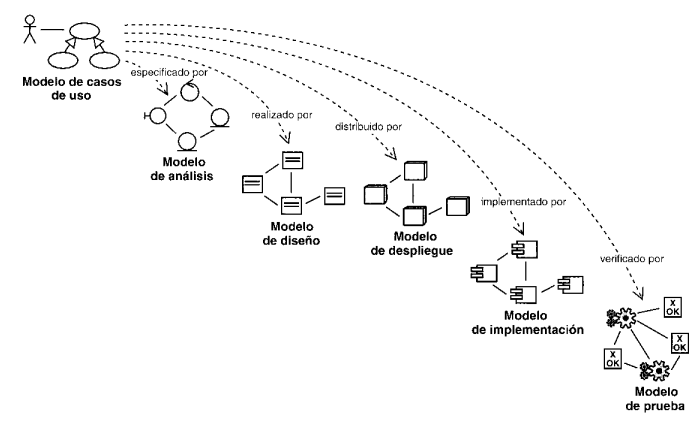
\includegraphics[width=0.8\textwidth]{/ciclofin.png} 
    \caption{Modelo del \acs{PUD} extraído de \cite{rumbaugh_jacobson_pud}.}
    \label{fig:ciclo-fin}
  \end{center}
\end{figure}


\begin{itemize}
\item \textbf{Modelo de casos de uso}: Todos los casos de uso del producto
  software. 
\item \textbf{Modelo de análisis}: Refina los casos de uso añadiendo más
  detalles y asigna funcionalidad a los objetos del producto software que
  proporcionan comportamiento.
\item \textbf{Modelo de diseño}: Define la estructura estática del sistema
  (subsistemas, clases e interfaces) que representan los casos de uso. 
\item \textbf{Modelo de implementación}: Incluye los componentes, que
  representan al código fuente así como la correspondencia entre las clases y
  esos dichos componentes.
\item \textbf{Modelo de despliegue}: Define los nodos físicos y su
  correspondencia con los componentes.
\item \textbf{Modelo de prueba}: Especifica los casos de prueba que verifican
  los casos de uso.
\item \textbf{Representación de la arquitectura}: Una representación de la
  arquitectura del sistema software desarrollado. 
\item El sistema debe tener un modelo de dominio o modelo del negocio. Su
  objetivo es describir el contexto del negocio en el que se encuentra el
  sistema. 
\end{itemize}


\subsubsection{Fases de un ciclo del Proceso Unificado de Desarrollo}

\cite{rumbaugh_jacobson_pud} cita y explica las cuatro fases de cada ciclo del \acs{PUD}:

\begin{enumerate}
\item Inicio
\item Elaboración
\item Construcción 
\item Transición
\end{enumerate}

A su vez, cada fase se puede descomponer a su vez en
iteraciones (véase figura \ref{fig:fases-ciclo}), acabando cada iteración en un hito. En la siguiente figura se
representa el esfuerzo que se realiza en cada una de las fases. 


\begin{figure}[!h]
  \begin{center}
    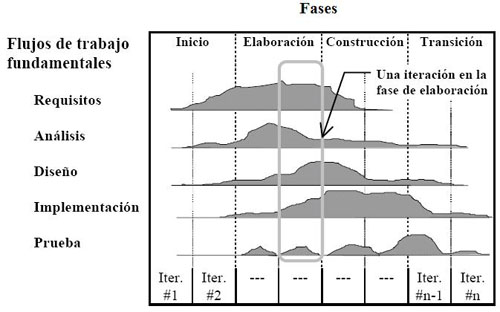
\includegraphics[width=0.8\textwidth]{/fases.jpg} 
    \caption{Diferentes fases del \acs{PUD} \cite{rumbaugh_jacobson_pud}.}
    \label{fig:fases-ciclo}
  \end{center}
\end{figure}



\textbf{Fase de Inicio}: En la fase de inicio se realiza una descripción del
producto final, es decir, se realiza el análisis de negocio para el producto
esperado. En esta fase se responde a las siguientes cuestiones: 

\begin{itemize}
\item Cuáles son las principales funciones del sistema para sus usuarios más
  importantes: lo que dará como resultado el modelo de casos de uso
  simplificado, conteniendo aquellos más críticos. 
\item Cómo podría ser la arquitectura del sistema: una vez se tiene el modelo,
  se comienza a esbozar la arquitectura con los subsistemas más importantes.

\item Cuál es el plan de proyecto y cuánto costará desarrollar el producto: del
  paso anterior se planifican los riesgos y comienza a estimarse el coste del
  proyecto. 
\end{itemize}


\textbf{Fase de Elaboración}: En esta fase se describe con más de talle los
casos de uso y se diseña de manera definitiva la arquitectura y el sistema al
completo. Finalmente, el director del proyecto debe ser capaz de planificar las
actividades y estimar los recursos necesarios para terminar el proyecto. 

\textbf{Fase de Construcción}: Fase de desarrollo del producto. El producto
final contiene todos los casos de uso que se han acordado para el sistema. La
línea base crecerá hasta convertirse en el sistema al completo. Se tiene una
arquitectura estable pero aún susceptible de mejorar. Puede no estar
completamente libre de defectos, que serán detectados y atajados en la fase de
transición. 

\textbf{Fase de Transición}: Corresponde al periodo en el cual el producto pasa
a ser una versión \textit{beta}. Se corrigen problemas y se realizan mejoras del
sistema. Además esta fase contiene otras actividades complementarias, tales
como formación del cliente, ayuda y asistencia, soporte técnico y corrección de
defectos. Estos defectos se pueden dividir en dos categorías: 

\begin{enumerate}
\item Los que tienen suficiente impacto para justificar un incremento. 
\item Los que pueden corregirse en una versión usual. 
\end{enumerate}



\section{Planificación del Proyecto}

En esta sección se muestra la planificación que se llevará a cabo en la
realización del \acs{TFM}. En el Capítulo \ref{chap:resultados} se detallarán
todos los productos resultantes de cada una de las iteraciones. 

El sistema software a desarrollar se describe a continuación. 

\subsection{SparkDQ: Un stack de Spark para la evaluación de la calidad de datos
  de triplas semánticas} 

Este capa software tendrá por objetivo resolver el problema del tratamiento de
datos semánticos en entornos Big Data. Se integrará e interactuará con el
framework Apache Spark para ofrecer un conjunto de primitivas de lectura de
datos semánticos y evaluación de la calidad de los mismos.

Este artefacto software tendrá las siguientes responsabilidades:

\begin{itemize}
\item Permitir la lectura de triplas semánticas y almacenarlas en una estructura
  de datos conveniente de forma distribuida.
\item Evaluación de los niveles de calidad de datos de un conjunto \acs{LOD}
  para la dimensión de calidad \textit{Completeness} desde la perspectiva de dos
  de sus métricas, descritas en su sección correspondiente del capítulo 3 (\ref{metricasdq}):
  \begin{itemize}
  \item \textit{Interlinking Completeness}
  \item \textit{Schema Completeness}
  \end{itemize}
\end{itemize}

\subsection{Prueba de Concepto para SparkDQ}

Para materializar el stack elaborado en el punto anterior, se elaborará una
aplicación software que aproveche las métricas implementadas en un caso de uso
real, en el que se tendrá una perspectiva \textit{end to end} de un problema de
calidad de datos, persiguiendo los siguientes objetivos:

\begin{enumerate}
\item Ingesta de datos semánticos en un entorno Big Data.
\item Evaluación de la calidad de los datos ingestados de manera distribuida. 
\item Almacenamiento de resultados de la evaluación.
\item Consumo de los resultados de la evaluación. 
\end{enumerate}

\subsection{Requisitos funcionales para SparkDQ}

Seguidamente se exponen los requisitos funcionales que se han identificado en la
primera fase del \acs{PUD}. Estos requisitos corresponden al desarrollo del
stack \textbf{SparkDQ}.

\begin{enumerate}
\item \textbf{SparkDQ debe permitir la carga de triplas semánticas en un entorno
  distribuido} \\La premisa inicial es que el volumen de datos es
  suficientemente grande como para que se requiera un almacenamiento y
  procesamiento en distribuido de los mismos. Por lo tanto, SparkDQ debe ser
  capaz de leer las triplas almacenadas en entornos distribuidos y cargarlas en
  un modelo igualmente distribuido para su posterior procesamiento.
  
\item \textbf{SparkDQ debe permitir al usuario modelar la evaluación de
  calidad}\\Se entiende como evaluación de calidad el cálculo de unas métricas y
  su posterior interpretación, así pues SparkDQ debe exponer mecanismos de
  evaluación de calidad de datos para ser llevados a cabo sobre un juego de
  datos distribuido. 
\item \textbf{SparkDQ debe permitir llevar a cabo evaluaciones de calidad de
  datos enlazados para la métrica \textit{SchemaCompleteness}}\\Se evaluará esta
  métrica considerando un esquema deseable para los datos obteniendo como
  resultado un grado de alineamiento de los datos con dicho esquema. 

\item \textbf{SparkDQ debe permitir llevar a cabo evaluaciones de calidad de
  datos enlazados para la métrica \textit{InterlinkingCompleteness}}\\Se
  evaluará esta métrica considerando un nivel de profundidad, siendo esto una
  agregación del nivel de interconectividad estratificado. 
\end{enumerate}

\subsection{Requisitos funcionales para la PoC}

Finalmente se exponen los requisitos funcionales identificados para la
aplicación de Prueba de Concepto.

\begin{enumerate}
\item \textbf{PoC debe permitir la adquisición de datos semánticos}\\Como parte
  del \textit{end to end} el primer paso de la prueba de concepto será
  seleccionar una fuente de datos y llevar a cabo un proceso de ingesta dentro
  de la arquitectura propuesta. 
  
\item \textbf{PoC debe permitir el almacenamiento de datos semánticos en un
  entorno distribuido}\\Los datos deben ingestarse en un entorno distribuido
  para su posterior consumo, considerando que su volumen y variedad pueden
  cambiar a lo largo del tiempo. 
\item \textbf{PoC debe permitir cargar datos semánticos desde un entorno
  distribuido y procesarlos}\\Los datos almacenados deben ser fácilmente
  accesibles y consumidos, entendiendo el consumo de estos datos como la
  adquisición, procesamiento y obtención de resultados en base a éstos. 
\item \textbf{PoC debe mantener unos niveles de seguridad adecuados}\\Los datos
  ingestados y almacenados deben estar protegidos de accesos no deseados. 
\item \textbf{PoC debe poder almacenar el resultado de las evaluaciones de
  calidad de datos en un entorno distribuido}\\Los resultados de las
  evaluaciones deben ser convenientemente almacenados bajo las mismas
  directrices de disponibilidad y seguridad que los datos inicialmente ingestados.
\item \textbf{PoC debe permitir el consumo de los resultados de las evaluaciones
  llevadas a cabo}\\Los resultados de las evaluaciones deben ser accesibles y
  fácilmente consumibles por parte de los usuarios. 
\end{enumerate}


\subsection{Iteraciones del \acs{PUD}}

La planificación del \acs{TFM} se desarrollará mediante iteraciones que
pertenecerán a diversas fases del Proceso Unificado de Desarrollo. En las
iteraciones más tempranas tendrá lugar la concepción del proyecto en lo que se
refiere a estudio, enlace con el \acs{PFC} y diseño de la solución. En las
iteraciones centrales el desarrollo y puesta a punto de los artefactos software
generados para finalmente, en la fase de transición del \acs{PUD}, la
elaboración de la prueba de conecpto y la entrega del presente trabajo. 


[INSERTA TABLA AQUÍ]

\subsubsection{Iteración 1: Planificación, casos de uso y requisitos}

Los objetivos de esta iteración son:

\begin{enumerate}

  \item Contextualizar el trabajo llevado a cabo en el \acs{PFC} con respecto a
  las tecnologías actuales y los avances en el campo.
\item Establecer una serie de casos de uso iniciales.
\item Fijar una serie de requisitos en base al conjunto de casos de uso
  especificado.
\item Establecer una arquitectura de la solución preliminar.

\end{enumerate}

Planteando este \acs{TFM} como una evolución del pasado \acs{PFC}, resulta
imprescindible conocer en qué punto se halla todo el trabajo realizado tras
varios años de evolución tecnológica. Es por lo tanto una de las iteraciones
cruciales para definir el rumbo del desarrollo así como de actualización del
estado de la cuestión.

Inicialmente se retoman las tecnologías utilizadas, Jena y JenaDQ, comprobando
su evolución en los últimos años. Seguidamente se establece un marco contextual
en el que se estudia el estado de la cuestión y se detectan carencias en el
ámbito actual: ausencia de frameworks que permitan el procesamiento distribuido
de triplas semánticas y el análisis de calidad de datos de las mismas en
entornos Big Data. 

Esto ayuda a especificar una serie de necesidades y unos casos de uso para
cubrirlas. En base a los casos de uso se generan los requisitos dirigidos
siempre hacia una arquitectura.

% Iteración 1
\vspace{1cm}
\begin{tabular}{|p{.2\textwidth}|p{.2\textwidth}|p{.4\textwidth}|}

\hline

\cellcolor[gray]{0.7}Fase del \acs{PUD} &
\cellcolor[gray]{0.7}Iteraciones &
\cellcolor[gray]{0.7}Objetivos \\
\hline
Inicio & Iteracion 1 &

\begin{itemize}
\item Estudiar el Estado del Arte.
\item Determinación del alcance del proyecto, requisitos y planificación.
\end{itemize}

\\
\hline

Elaboracion & Iteración 2 &

\begin{itemize}

\item Actualización técnica de JenaDQ.
\end{itemize}

\\
& Iteración 3 &


\begin{itemize}
\item Diseño de la arquitectura de SparkDQ: Dependencia con SparkRDF y Jena.
\end{itemize}
\\
\hline


Construcción & Iteración 4 &


\begin{itemize}
\item Análisis, Diseño, Implementación y Pruebas para SparkRDF.
\end{itemize}
\\
& Iteración 5 &

\begin{itemize}
\item Análisis, Diseño, Implementación y Pruebas para SparkDQ: \textit{Interlinking}.
\end{itemize}
\\
& Iteración 6 &

\begin{itemize}
\item Análisis, Diseño, Implementación y Pruebas para SparkDQ: \textit{SchemaCompleteness}.
\end{itemize}
\\
\hline
Transición & Iteración 7 &

\begin{itemize}
\item Análisis, Diseño, Implementación y Pruebas para \acs{PoC}.
\end{itemize}
\\
& Iteración 8 &

\begin{itemize}
\item Entrega \acs{TFM}
\end{itemize}
\\
\hline

\end{tabular}
\captionof{table}{Resumen de iteraciones para \acs{PUD}}


% Local variables:
%   coding: utf-8
%   ispell-local-dictionary: "castellano8"
%   TeX-master: "main.tex"
% End:


\subsubsection{Iteración 2: Actualización de JenaDQ}

Una vez establecidos los requisitos, se dispone a actualizar el estado de JenaDQ
para dotarle de mayor nivel de madurez y alinearlo al trabajo que va a ser
desarrollado, de manera que pueda compararse en ejecución con los desarrollos
que van a tener lugar. 

[INSERTA TABLA AQUÍ]

\subsubsection{Iteración 3: Diseño de arquitectura de SparkDQ}

Tras analizar la problemática comienza el diseño de las soluciones. En este
caso, el objetivo final es elaborar un stack que permita el procesamiento
distribuido de triplas semánticas y la evaluación de la calidad de datos de las
mismas de manera escalable. Para ello se requerirán de dos artefactos:

\begin{enumerate}
\item \textbf{SparkRDF}: como interfaz entre un conjunto suficientemente grande de
  triplas semánticas y una representación escalable que permita la
  transformación de éstas hacia modelos de procesamiento distribuido, en este
  caso y como se verá en el capítulo de resultados, mediante un grafo dirigido.
\item \textbf{SparkDQ}: Una vez se tenga la representación distribuida de las triplas, se
  procederá a la creación de primitivas que permitan la evaluación de la calidad
  de los datos para las métricas \textit{SchemaCompleteness} e \textit{Interlinking}.
\end{enumerate}


El objetivo de esta iteración será diseñar los componentes necesarios para dar
soporte al desarrollo de estos dos artefactos.

[INSERTA TABLA AQUÍ]


\subsubsection{Iteración 4: Desarrollo de SparkRDF}

Una vez diseñada la arquitectura, comienza el desarrollo con su primera
dependencia: obtención de datos semánticos y representación en estructuras de
datos distribuídas propias del framework de desarrollo.

Para ello se abordan las etapas tradicionales de desarrollo: Análisis, Diseño,
Implementación y Pruebas. Se iterará hasta que se estime un estado óptimo del
artefacto. 

[INSERTA TABLA AQUÍ]

\subsubsection{Iteración 5: Desarrollo de SparkDQ: Evaluación
  \textit{Interlinking}}

Teniendo el punto de entrada de los datos, lo siguiente es comenzar con la
elaboración del artefacto de evaluación de calidad de datos mediante
métricas.

La primera iteración sobre este artefacto tendrá por objetivo la elaboración de
el conjunto de funciones necesarias para implementar la métrica
\textit{Interlinking}.

Se abordará mediante las etapas tradicionales: Análisis, Diseño,
Implementación y Pruebas, iterando hasta que el resultado sea óptimo. 

[INSERTA TABLA AQUÍ]


\subsubsection{Iteración 6: Desarrollo de SparkDQ: Evaluación
  \textit{SchemaCompleteness}}


La segunda iteración sobre este artefacto tendrá por objetivo la elaboración de
el conjunto de funciones necesarias para implementar la métrica
\textit{SchemaCompleteness}.

Se abordará mediante las etapas tradicionales: Análisis, Diseño,
Implementación y Pruebas, iterando hasta que el resultado sea óptimo. 

[INSERTA TABLA AQUÍ]

\subsubsection{Iteración 7: Desarrollo de la PoC}

Finalmente tras haber finalizado el artefacto de evaluación de la calidad, se
aplicará sobre una prueba de concepto. Esta prueba a su vez se dividirá en una
serie de fases de Análisis, Diseño, Implementación y Pruebas, no relativas
únicamente al artefacto software a desarrollar, sino a la arquitectura global
que se ofrecerá finalmente. 

[INSERTA TABLA AQUÍ]


\subsubsection{Iteración 8: Entrega de \acs{TFM}}

Una vez realizada la prueba de concepto, se finaliza el trabajo pendiente
redactando y detallando la documentación:

\begin{enumerate}
\item Memoria del \acs{TFM}
\item Documentación sobre los distintos artefactos generados:
  \begin{itemize}
  \item SparkRDF
  \item SparkDQ
  \item spark-sem-dq-assessment
  \item Microservicio de ingesta
  \item Microservicio de transformación tweets a triplas semánticas
  \item Ontologías desarrolladas
  \end{itemize}
\end{enumerate}

[INSERTA TABLA AQUÍ]

\section{Marco tecnológico de trabajo}

\label{sec:marcotrabajo}

En esta sección se describen las herramientas y tecnologías que se han elegido
para dar soporte al desarrollo de este \acs{TFM}. Dichas herramientas y tecnologías
son utilizadas tanto para el modelado del sistema y desarrollo de diagramas como
para la implementación del código y la documentación necesaria. 

\subsection{Frameworks de desarrollo de aplicaciones de Web (Semántica)}

Los distintos frameworks utilizados durante la elaboración de este \acs{TFM} se
exponen a continuación. 

\begin{definitionlist} 

\item[Apache Jena]

Jena (\url{http://jena.apache.org}) es un framework de código abierto, basado en
Java para la construcción de aplicaciones basadas en tecnología Semántica y
datos enlazados. 

En el Capítulo \ref{chap:estadoarte} se han explicado algunas de las
características más importantes de este framework. 

\item[Apache Spark]

  Spark (\url{http://spark.apache.org}) se ha convertido en el estándar
  \textit{de facto} a la hora del procesamiento distribuido de alta velocidad.

  En el Capítulo \ref{chap:estadoarte} se han explicado las características más
  interesantes de dicho framework así como la importancia que tiene en el actual
  ecosistema Big Data. 

\end{definitionlist}

\subsection{Software de Desarrollo}

Como software de soporte al desarrollo del \acs{TFM} se han utilizado las
siguientes herramientas. 

\begin{definitionlist} 
\item[IntelliJ]

  IntelliJ (\url{https://www.jetbrains.com/idea/}) es un \acf{IDE} que ha ganado
  en popularidad durante los últimos años debido a su extensibilidad y facilidad
  de uso. Puede enriquecerse con \textit{plugins} que dan soporte a tecnologías
  actuales y facilitan la experiencia de desarrollo. 


\item[Visual Paradigm]

  Visual Paradigm (\url{http://www.visual-paradigm.com}) es una herramienta
  \acf{CASE} que permite facilitar todo el proceso de desarrollo, incluyendo
  herramientas de edición de diagramas \acs{UML} de todo tipo y generación de
  código automática a partir de diagramas y viceversa. 

  Visual Paradigm se ha utilizado para la realización de todos los diagramas. 

\item[Git]

  
  Git (\url{http://git-scm.com/}) ha sido el software de control de versiones
  utilizado para el desarrollo. 

\item[jUnit]

  jUnit (\url{http://junit.sourceforge.net}) es un framework que permite realizar
  ejecución de pruebas unitarias de manera controlada para evaluar el correcto
  funcionamiento de determinado código. 

\item[Protégé]

  Protégé (\url{http://protege.stanford.edu}) es un editor de ontologías de código
  abierto. Se ha utilizado en este proyecto para la creación del vocabulario de
  evaluación de calidad de datos. 

\end{definitionlist}


\subsection{Edición}

Para las diferentes labores de edición, tanto de texto como de imagen, se han
utilizado las siguientes herramientas. 

\begin{definitionlist} 
\item[\LaTeX]

  \LaTeX es un sistema de composición de textos orientado principalmente a la
  creación de documentos científicos y técnicos. 

  Toda la documentación se ha generado con esta tecnología. 

\item[BibTeX]
  BibTeX es un sistema gestor de referencias bibliográficas que se integra con
\LaTeX.

\item[Emacs]

  Emacs (\url{www.gnu.org/software/emacs/}) es un editor de texto multifuncional
  que incluye una gran cantidad de librerías y extensiones para facilitar
  cualquier tipo de edición que se lleve a cabo sobre él. 

  En este proyecto, se ha utilizado Emacs integrado con \LaTeX para la
  elaboración de toda la documentación. También para la edición de otros archivos
  menores como reglas o scripts. 

\item[Dia]

  Dia (\url{https://wiki.gnome.org/Apps/Dia}) es un programa editor de diagramas
  de diferentes tipos (\acs{UML}, flujo de datos, \ldots). 

\item[Gimp]

  
  Gimp (\url{www.gimp.org}) es un editor de imagen de código abierto. 

\end{definitionlist}

\subsection{Servidores}

Se han utilizado dos tipos de servidores: los de la aplicación Web y los de
datos. Se enumeran a continuación. 

\begin{definitionlist} 
\item[Apache Tomcat]

Apache Tomcat (\url{http://tomcat.apache.org}) es un servidor Web de código
abierto para aplicaciones Java. 

\item[Jena TDB]

Dentro del proyecto Jena, TDB es sistema de almacenamiento altamente escalable y
de alta velocidad empleado para las triplas. 


\item[Jena Fuseki]

Dentro del proyecto Jena, Fuseki es el servidor de triplas sobre el que se
pueden realizar consultas como endpoint a través del protocolo \acs{HTTP}. Se
integra sobre distintos servidores pero principalmente sobre TDB. 

\end{definitionlist}

\subsection{Cloud computing}

Se han utilizado diversas soluciones \textit{cloud} para llevar a cabo el
desarrollo de la prueba de concepto. En este caso, el proveedor elegido ha sido
Amazon Web Services, utilizando los siguientes servicios:

\begin{itemize}

\item \textbf{Amazon S3}: \textit{Simple Storage Service} o S3 es un servicio de almacenamiento
  distribuido y escalable basado en \textit{buckets} como directorios.
  
\item \textbf{Amazon Elastic Search}: Solución de Amazon para un servicio autogestionado del stack ElasticSearch y
  Kibana. ElasticSearch es un indexador de documentos basado en índices,
  mientras que Kibana, montado sobre éste, permite visualizar los documentos
  indexados a través de agregaciones sencillas. 
\end{itemize}

\subsection{Lenguajes de Programación}

A continuación se indican aquellos lenguajes de programación que han tenido más
peso en el desarrollo del \acs{TFM}. 

\begin{definitionlist} 

\item[Java]

Java (\url{https://www.java.com/}) es el lenguaje de programación para el
desarrollo de la parte central del proyecto. Se ha escogido Java debido a su
gran extensión y soporte por parte de la comunidad. 

Para este \acs{TFM} se ha trabajado con la versión 1.8.

\item[Scala]

  Scala(\url{https://www.scala-lang.org/}) es un lenguaje de programación
  funcional, que está convirtiéndose en una auténtica revolución en el mundo del
  Big Data debido a que corre sobre la máquina virtual de Java, permite
  reutilizar todas las librerías disponibles para éste y su orientación
  funcional lo hace idóneo para la resolución de problemas y elaboración de
  algoritmos en estos ámbitos. Es el lenguaje con el
  que está desarrollado Spark y ha sido el lenguaje de programación con el que
  se ha desarrollado el grueso del proyecto. La versión utilizada para el desarrollo de este
  \acs{TFM} es la 2.11.


\item[Datalog Jena]

Para la parte relacionada con la inferencia, Jena posee su propio lenguaje de
definición de reglas: Datalog Jena. Es el lenguaje utilizado para definir las
reglas de contexto que luego se han utilizado para llevar a cabo los
razonamientos (véase Sección \ref{sec:eajena}). 



\item[\acs{SPARQL}]

\acs{SPARQL} es el lenguaje declarativo para llevar a cabo operaciones de
consulta y actualización sobre conjuntos de datos semánticos. 

\end{definitionlist}

\subsection{Equipos de desarrollo}

Para la realización del \acs{TFM} se han utilizado las siguientes máquinas: 

\begin{itemize}
\item PC con \textit{GNU/Linux Ubuntu 16.04} procesador Intel i7
  de ocho núcleos de 2.6 GHz y 16 GB de RAM.
\item PC con \textit{GNU/Linux Ubuntu 16.04} procesador Intel i5
  de cuatro núcleos de 2.6 GHz y 16 GB de RAM.   
\end{itemize}
